\documentclass[aspectratio=169]{beamer}

\usepackage[T1]{fontenc}
\usepackage[utf8]{inputenc}
\usepackage{lmodern}
\usepackage{graphicx}
\usepackage{xcolor}
\usepackage{booktabs}

\graphicspath{{images_benchmark_types/}{images_datasets/}}

\definecolor{accent}{RGB}{37,96,151}
\definecolor{soft}{RGB}{237,243,248}
\definecolor{ink}{RGB}{32,44,58}

\usetheme{Madrid}
\usecolortheme{default}
\setbeamercolor{structure}{fg=accent}
\setbeamercolor{frametitle}{fg=white,bg=accent}
\setbeamercolor{title}{fg=white,bg=accent}
\setbeamercolor{normal text}{fg=ink}
\setbeamertemplate{navigation symbols}{}

\title{Vision-Language Benchmarking}
\subtitle{Short Beamer Example}
\author{Samuel}
\date{\today}

\begin{document}

\begin{frame}
  \titlepage
\end{frame}

\begin{frame}{Motivation}
  \begin{itemize}
    \item Modern vision-language models can caption, classify, answer questions, detect objects, and compare images.
    \item A single leaderboard hides differences between task families.
    \item A benchmark harness makes heterogeneous datasets comparable under one evaluation pipeline.
  \end{itemize}
\end{frame}

\begin{frame}{Benchmark Types}
  \begin{table}
    \centering
    \small
    \begin{tabular}{lll}
      \toprule
      Type & Task & Example dataset \\
      \midrule
      C & Captioning & Conceptual Captions \\
      A & Visual QA & FlyingThings3D \\
      B & Detection & MS COCO \\
      R & Rating & TAD66K \\
      P & Preference & Pick-a-Pic \\
      \bottomrule
    \end{tabular}
  \end{table}
\end{frame}

\begin{frame}{Example Input}
  \begin{columns}[T]
    \begin{column}{0.54\textwidth}
      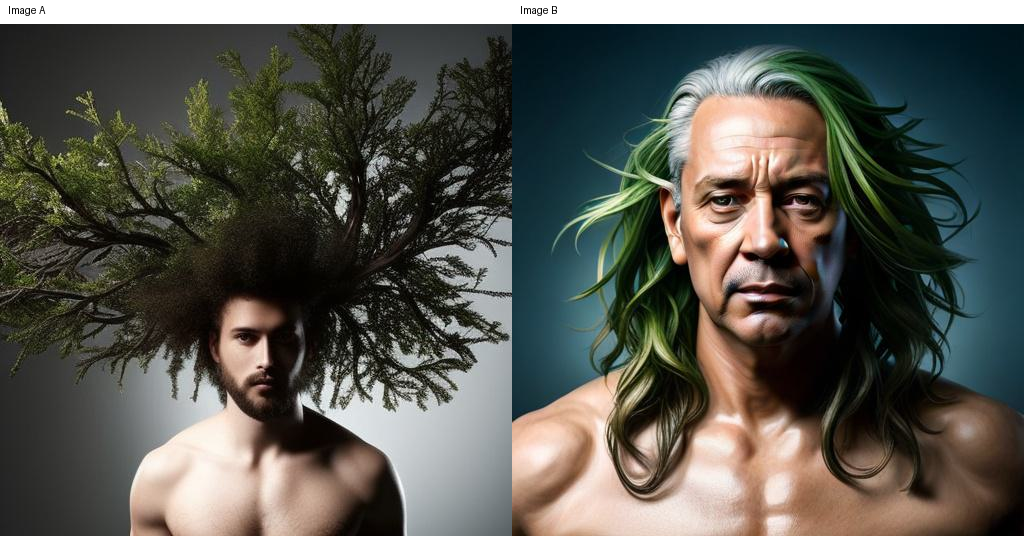
\includegraphics[width=\textwidth]{type_p_pick_a_pic_04.png}
    \end{column}
    \begin{column}{0.42\textwidth}
      \textbf{Prompt}

      Which image is more aesthetically pleasing overall?

      \vspace{0.6em}
      A. Image A

      B. Image B

      \vspace{1em}
      \textbf{GPT-4o response:} A

      \textbf{Reference:} Image A
    \end{column}
  \end{columns}
\end{frame}

\begin{frame}{Takeaway}
  \begin{block}{Main idea}
    The harness should record both quality and failure behavior: predictions,
    parsed answers, references, errors, runtime, and task-specific metrics.
  \end{block}

  \vspace{0.8em}
  This makes model comparisons auditable rather than only producing a final score.
\end{frame}

\end{document}
